\documentclass[hyperref=colorlinks]{beamer}
\mode<presentation>
\usetheme{iclpt}
\setbeamertemplate{navigation symbols}{}
\setbeamertemplate{headline}{
\begin{beamercolorbox}[leftskip=.2cm,rightskip=.2cm,topskip=.2cm,ht=1.1cm,dp=0.1cm,wd=\textwidth]{institute in head/foot}
  
\includegraphics[height=1cm]{icl.pdf}
  \hfill
  
\includegraphics[height=1cm]{../Pics/CMS-Color.pdf}
\end{beamercolorbox}
}
\setbeamertemplate{footline}{
\begin{beamercolorbox}[ht=.55cm,dp=0.4cm,wd=\textwidth,leftskip=.3cm]{author in head/foot}%
  \begin{minipage}[c]{5cm}%
    \usebeamerfont{author in head/foot}
    \insertshortauthor 
    \insertshorttitle
    \end{minipage}\hfill%
  \insertframenumber{} / \pageref{lastframe}
  \hfill
  \begin{minipage}{6cm}
    \hfill
  \end{minipage}
\end{beamercolorbox}%
}

\usepackage{color}
\usepackage{tabularx,colortbl}
\usepackage{graphicx}
\usepackage{pdfpages}
\usepackage{feynmp}
\usepackage{tikz}
\usetikzlibrary{calc, shapes, backgrounds,arrows,positioning}
\DeclareGraphicsRule{*}{mps}{*}{}

\title{\vspace{-0.2cm} VBF Higgs to Invisible}
\subtitle{HIG-14-038, AN-14-243\vspace{-0.7cm}}
\author[]{}%\underline{P. Dunne}} % A.M. Magnan and A. Nikitenko Joao Pela with \\ R. Aggleton, J. Brooke: Bristol \\ C.Asawangtrakuldee, Q.Li: Peking \\ P. Srimanobhas: Chulalongkorn \\ S. Kumar, K. Mazumdar: Mumbai}
\titlegraphic{
  \vspace{-0.7cm}
  %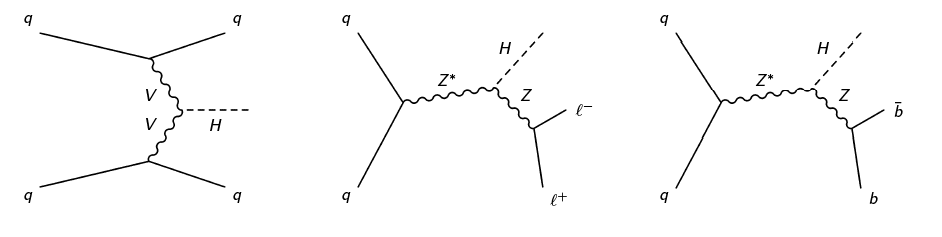
\includegraphics[width=\textwidth]{TalkPics/invcomb021213/feyndiags}
  %% \begin{fmfgraph*}(100,70)
  %%         \fmfleft{i1,i2}
  %%         \fmfright{o1,o2,o3}
  %%         \fmf{fermion}{i1,v1,o1}
  %%         \fmf{fermion}{i2,v2,o3}
  %%         \fmf{phantom,tension=4/5}{v1,v2}
  %%         \fmffreeze
  %%         \fmf{photon,label=$W,,Z$}{v1,v3}
  %%         \fmf{photon,label=$W,,Z$}{v2,v3}
  %%         \fmf{dashes}{v3,o2}
  %%         \fmflabel{$q$}{i1}
  %%         \fmflabel{$q$}{i2}
  %%         \fmflabel{$q$}{o1}
  %%         \fmflabel{$q$}{o3}
  %%         \fmflabel{$H$}{o2}
  %%       \end{fmfgraph*}
}
\date{}
\begin{document}
\begin{fmffile}{higgsexoupdatefeyndiags}
\tikzstyle{every picture}+=[remember picture]

%TITLE PAGE
\section{Title}
\begin{frame}
  \titlepage
  
\end{frame}

\begin{frame}
  \frametitle{Reminder of status at the beginning of the week}
  \begin{block}{}
    \begin{itemize}
    \item All objects have at least a basic recipe in our ntuples
    \item ak4 non-CHS jets and MET need most work
    \item First production of signal and QCD samples completed
    \end{itemize}
    \end{block}
\end{frame}

\begin{frame}
  \frametitle{Technical Progress}
  \begin{block}{}
    \begin{itemize}
    \item We have a new twiki \href{https://twiki.cern.ch/twiki/bin/view/CMS/VBFHinvisibleRun2}{here}
    \item Change to storage of MET in ntuples necessitated separate run 2 LightTreeMaker and rerunning of ntuples
    \item[-] New production is May20
    \item[-] Light tree making scripts now use run2 light tree maker by default
    \item Light trees for run 2 signal samples now made
    \end{itemize}
  \end{block}
\end{frame}

\begin{frame}
  \frametitle{Signal comparison: run 1 vs run 2}
  \begin{block}{}
    \begin{itemize}
    \item Use $m_{H}$=125 GeV samples with a range of conditions
    \item Start with parked analysis signal region:
      $\eta_{j1} \cdot \eta_{j2}<0,\, \eta_{j1}<4.7,\, \eta_{j2}<4.7,$
      $p_{T}^{\text{j1}}>50 \,\text{GeV},\,p_{T}^{\text{j2}}>45\,\text{GeV},$
      $\Delta\eta_{jj}>3.6,\, M_{jj}>1200\,\text{GeV},$
      $MET>90\,\text{GeV},$
      $mindphiall > 2.3,\, METsig>4.$
    \item[-] Plan to look at other regions as well
    \item Trigger weighting etc. as in parked analysis
    \item[-] Obviously will need updating for real analysis
    \item All distributions normalised to 1
    \item Data/Bkg is Run 2 PU20BX25/Run 1
    \end{itemize}
  \end{block}
\end{frame}

\begin{frame}
  \frametitle{Signal comparison: run 1 vs run 2: Jet $p_{T}$}
  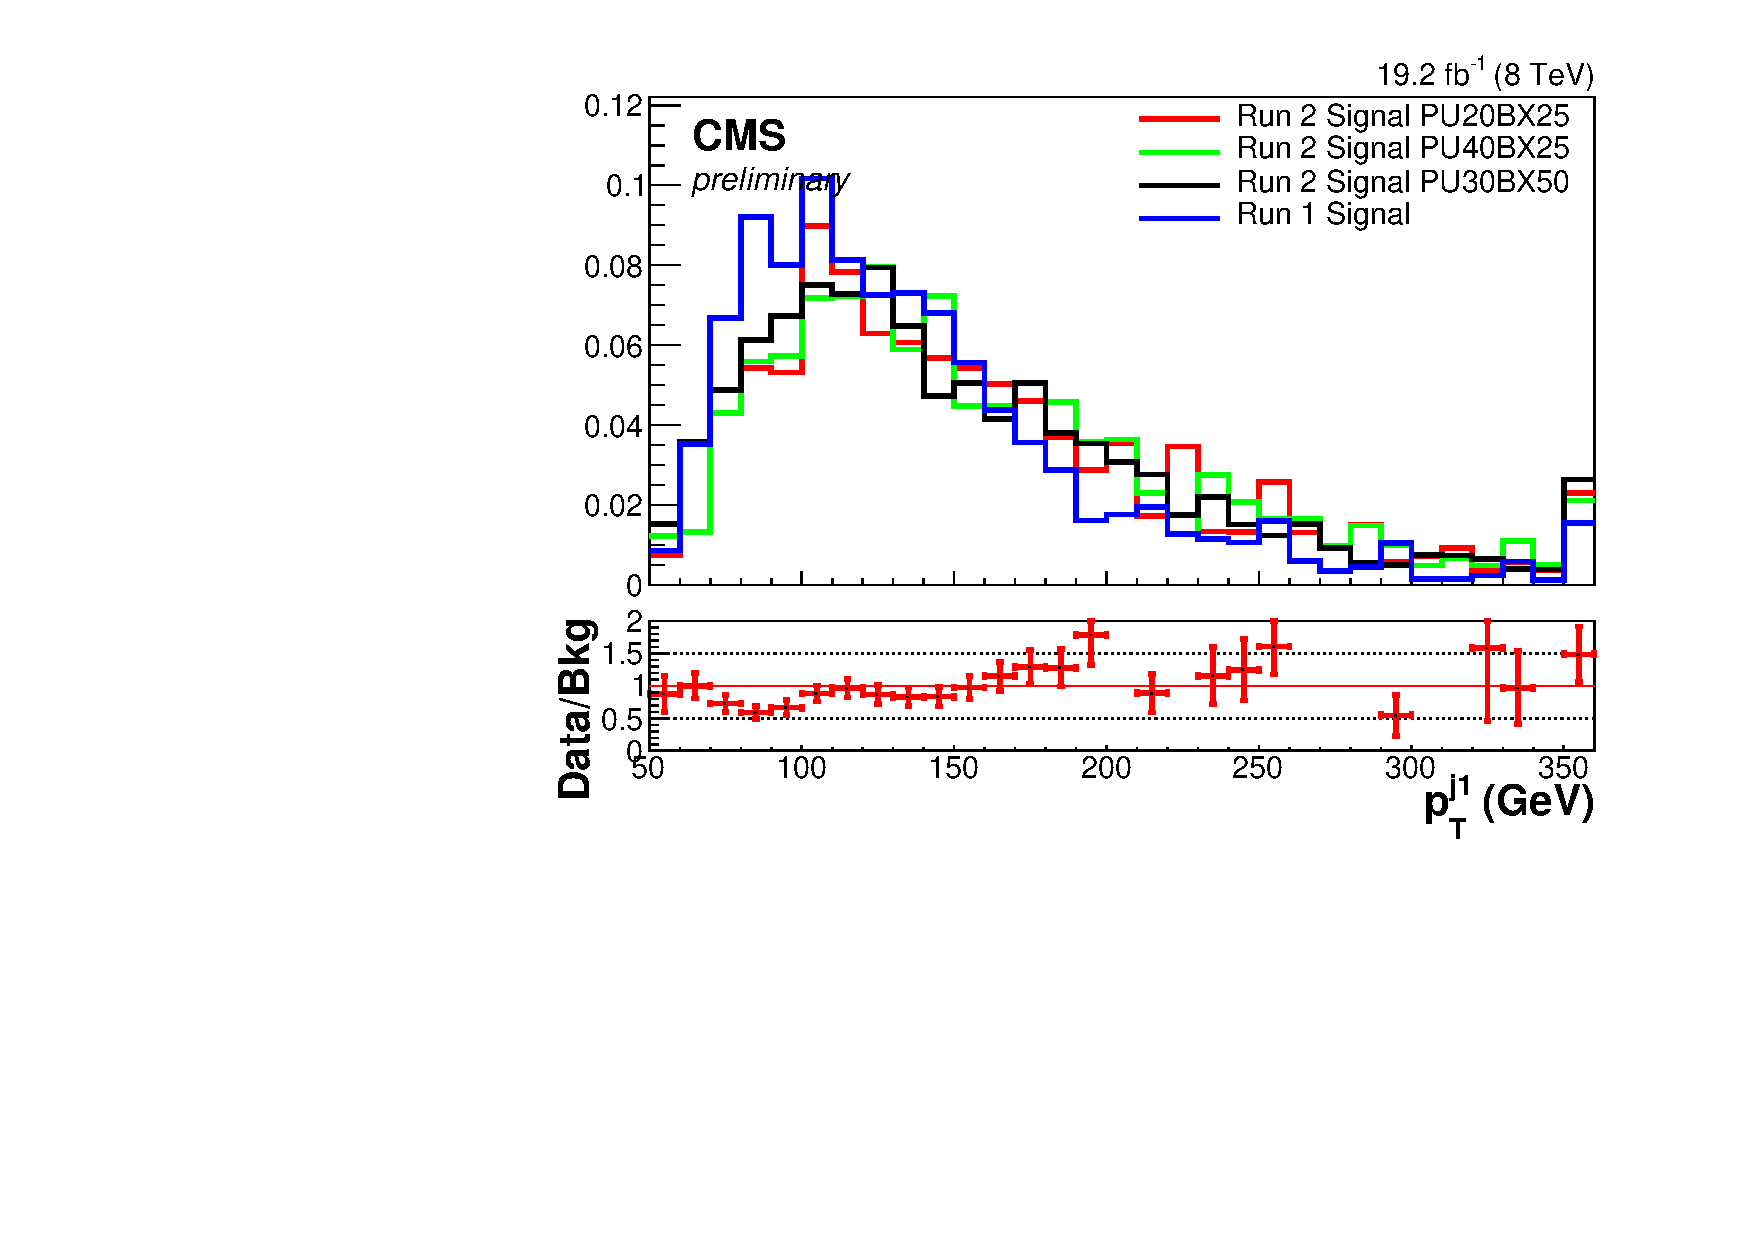
\includegraphics[width=.5\textwidth]{TalkPics/firstrun2mccontrolplots/output/nunu_norm_jet1_pt.pdf}
  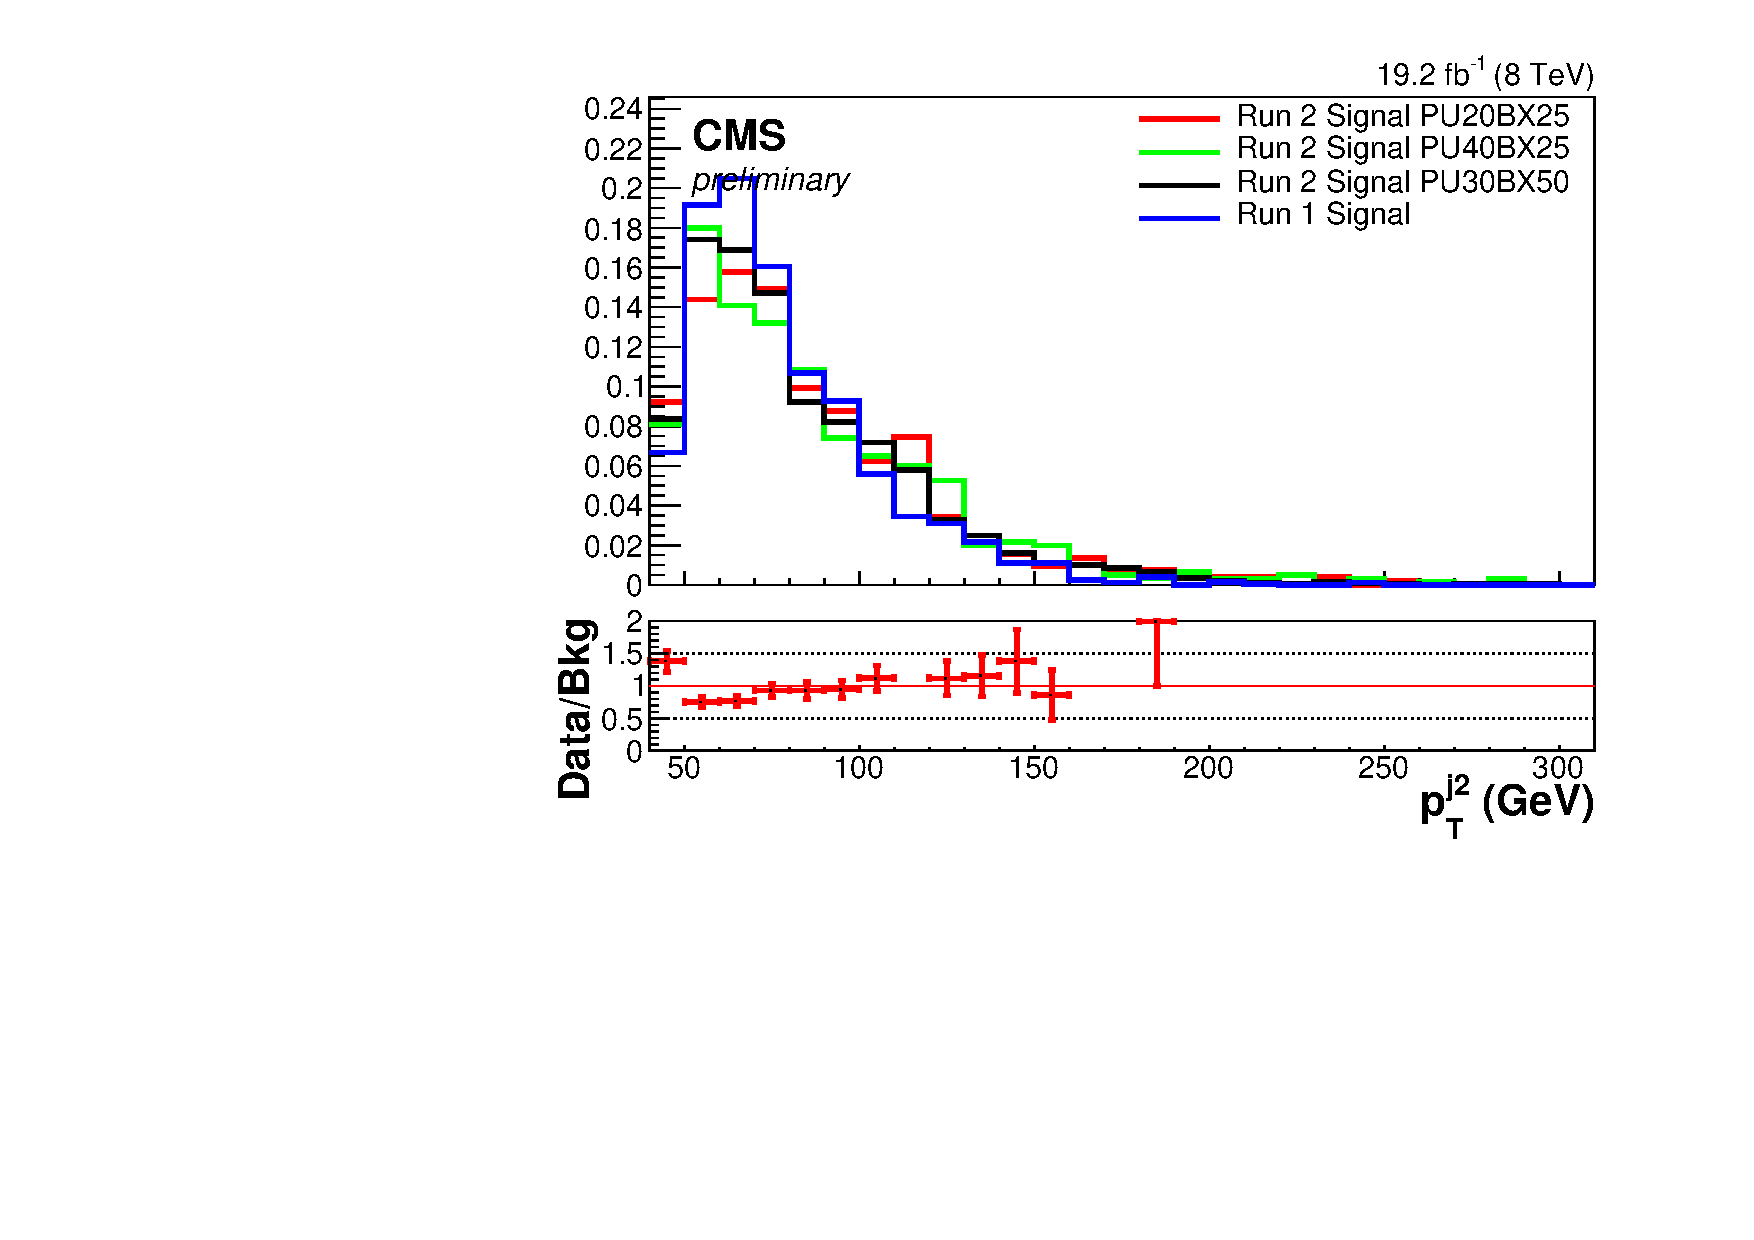
\includegraphics[width=.5\textwidth]{TalkPics/firstrun2mccontrolplots/output/nunu_norm_jet2_pt.pdf}
  \begin{block}{}
    \begin{itemize}
    \item[-] Jets in run 2 (red, green, black) have generally higher $p_T$ than those in run 1 (blue)
    \end{itemize}
  \end{block}
\end{frame}

\begin{frame}
  \frametitle{Signal comparison: run 1 vs run 2: Jet $\eta$}
  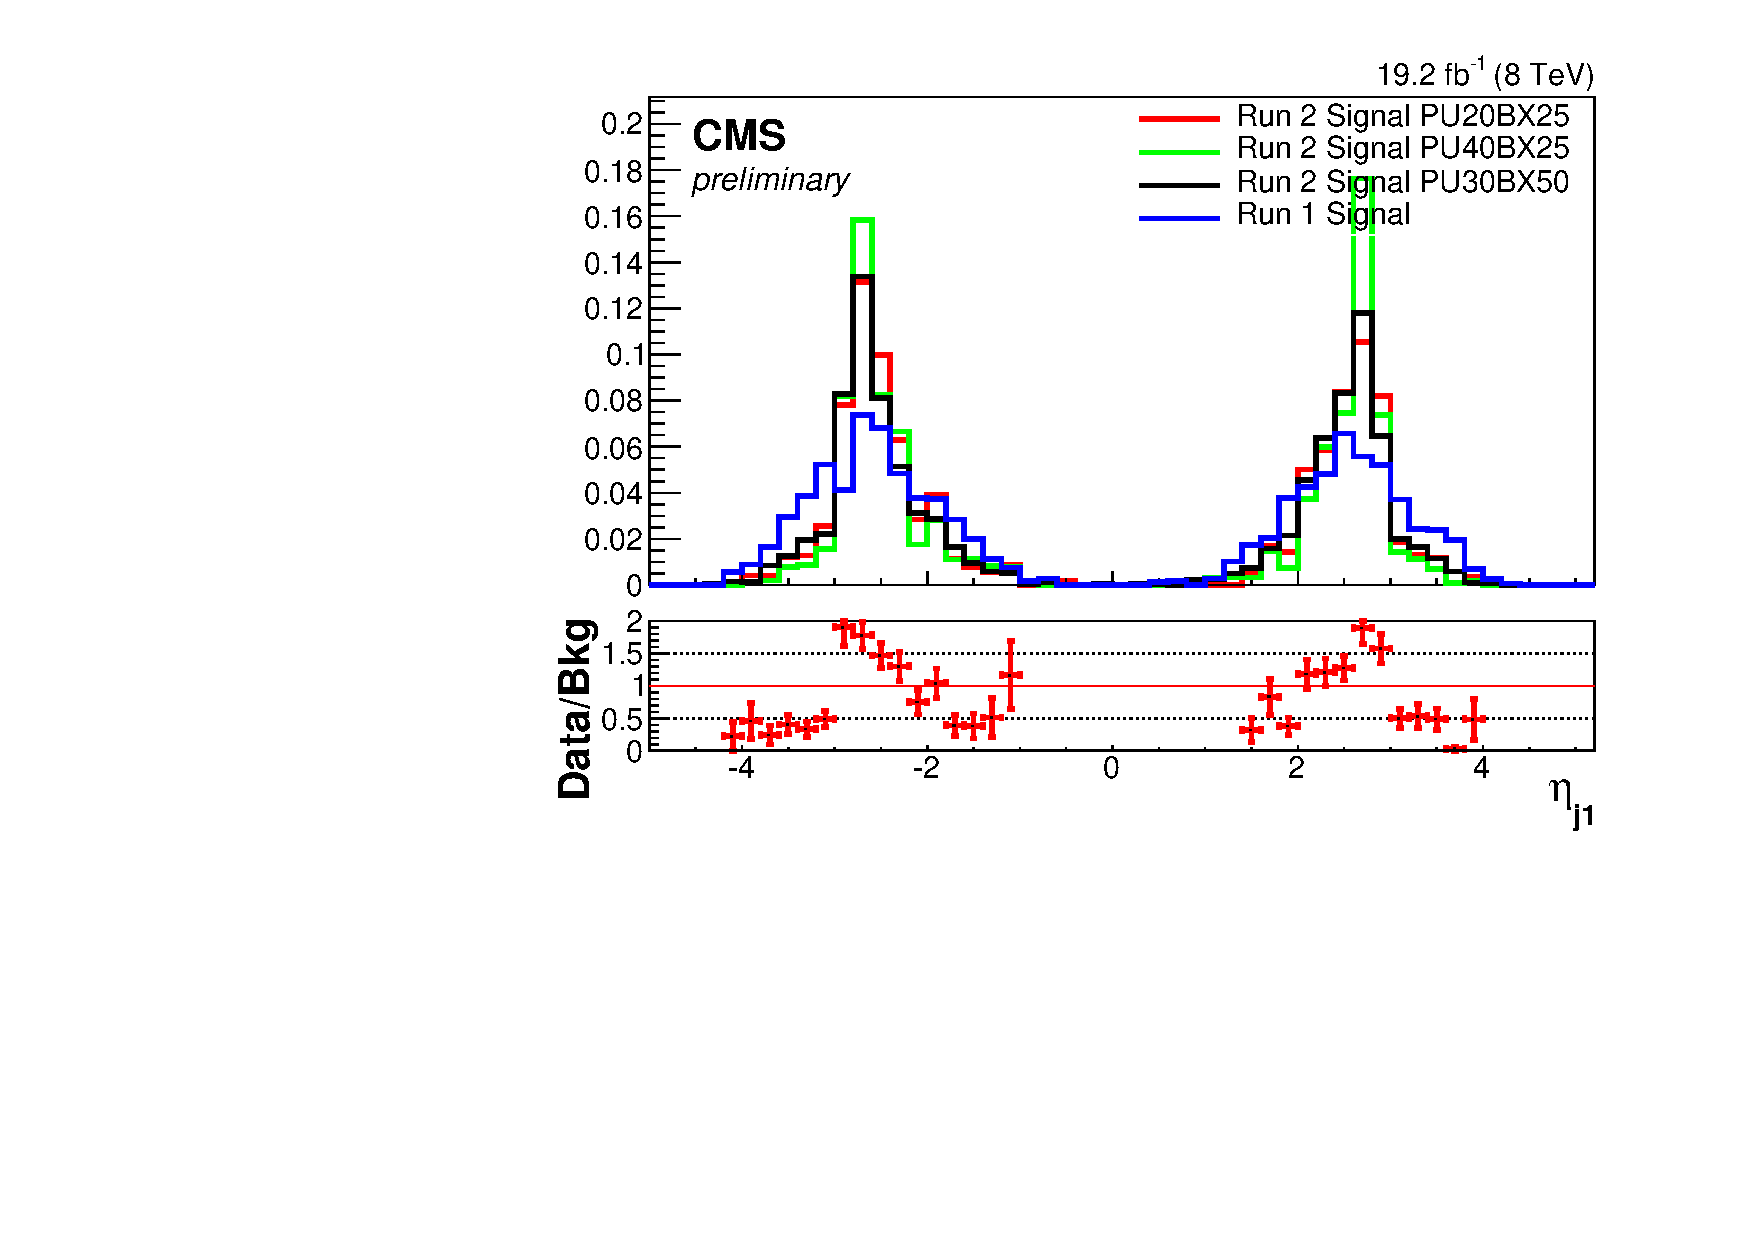
\includegraphics[width=.5\textwidth]{TalkPics/firstrun2mccontrolplots/output/nunu_norm_jet1_eta.pdf}
  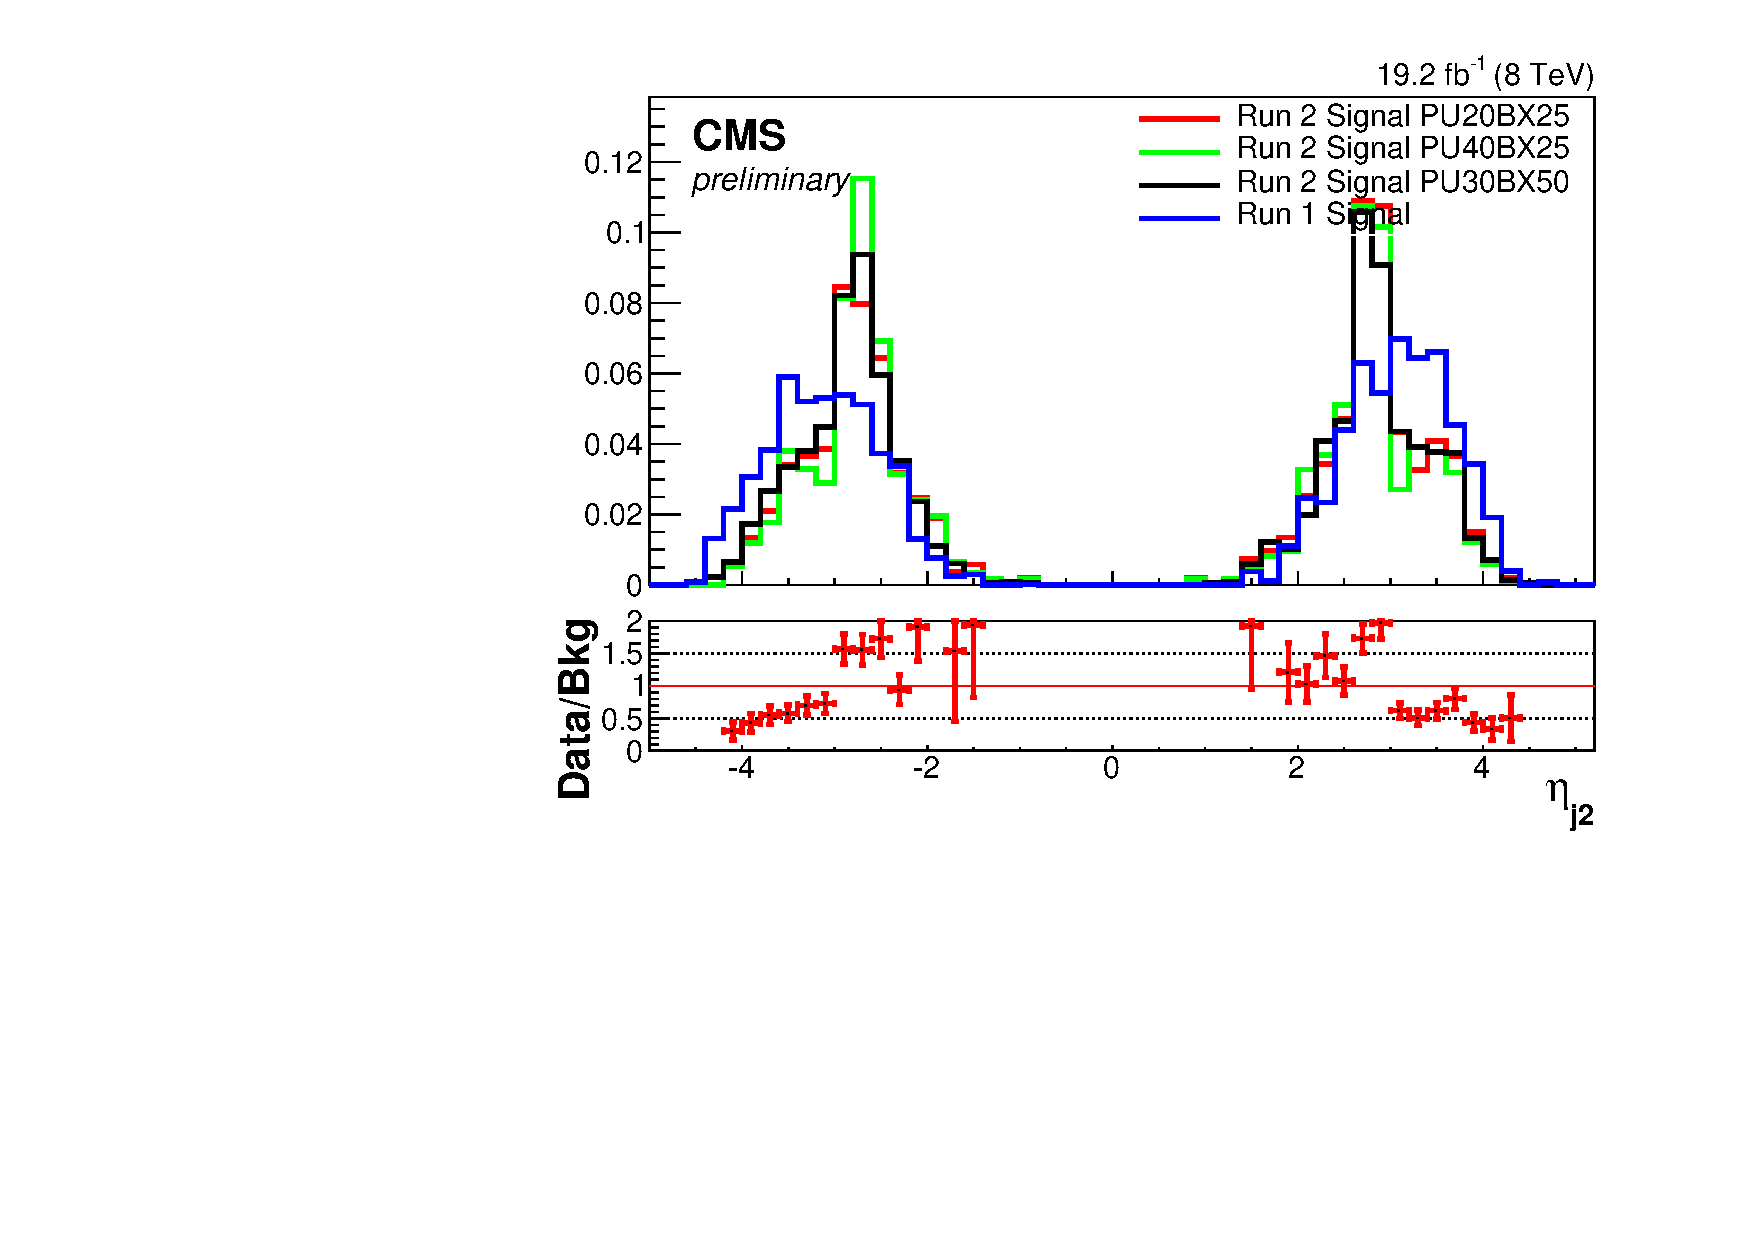
\includegraphics[width=.5\textwidth]{TalkPics/firstrun2mccontrolplots/output/nunu_norm_jet2_eta.pdf}
  \begin{block}{}
    \begin{itemize}
    \item Run 2 jet $\eta$ has spike from 2.5-3
    \item These ``ears'' are a known feature also seen by $H\rightarrow\gamma\gamma$ and are due to barrel-endcap transition and end of tracker coverage
    \item Better calibration expected in 7\_4\_2
    \end{itemize}
  \end{block}
\end{frame}

\begin{frame}
  \frametitle{Signal comparison: run 1 vs run 2: Jet $\phi$}
  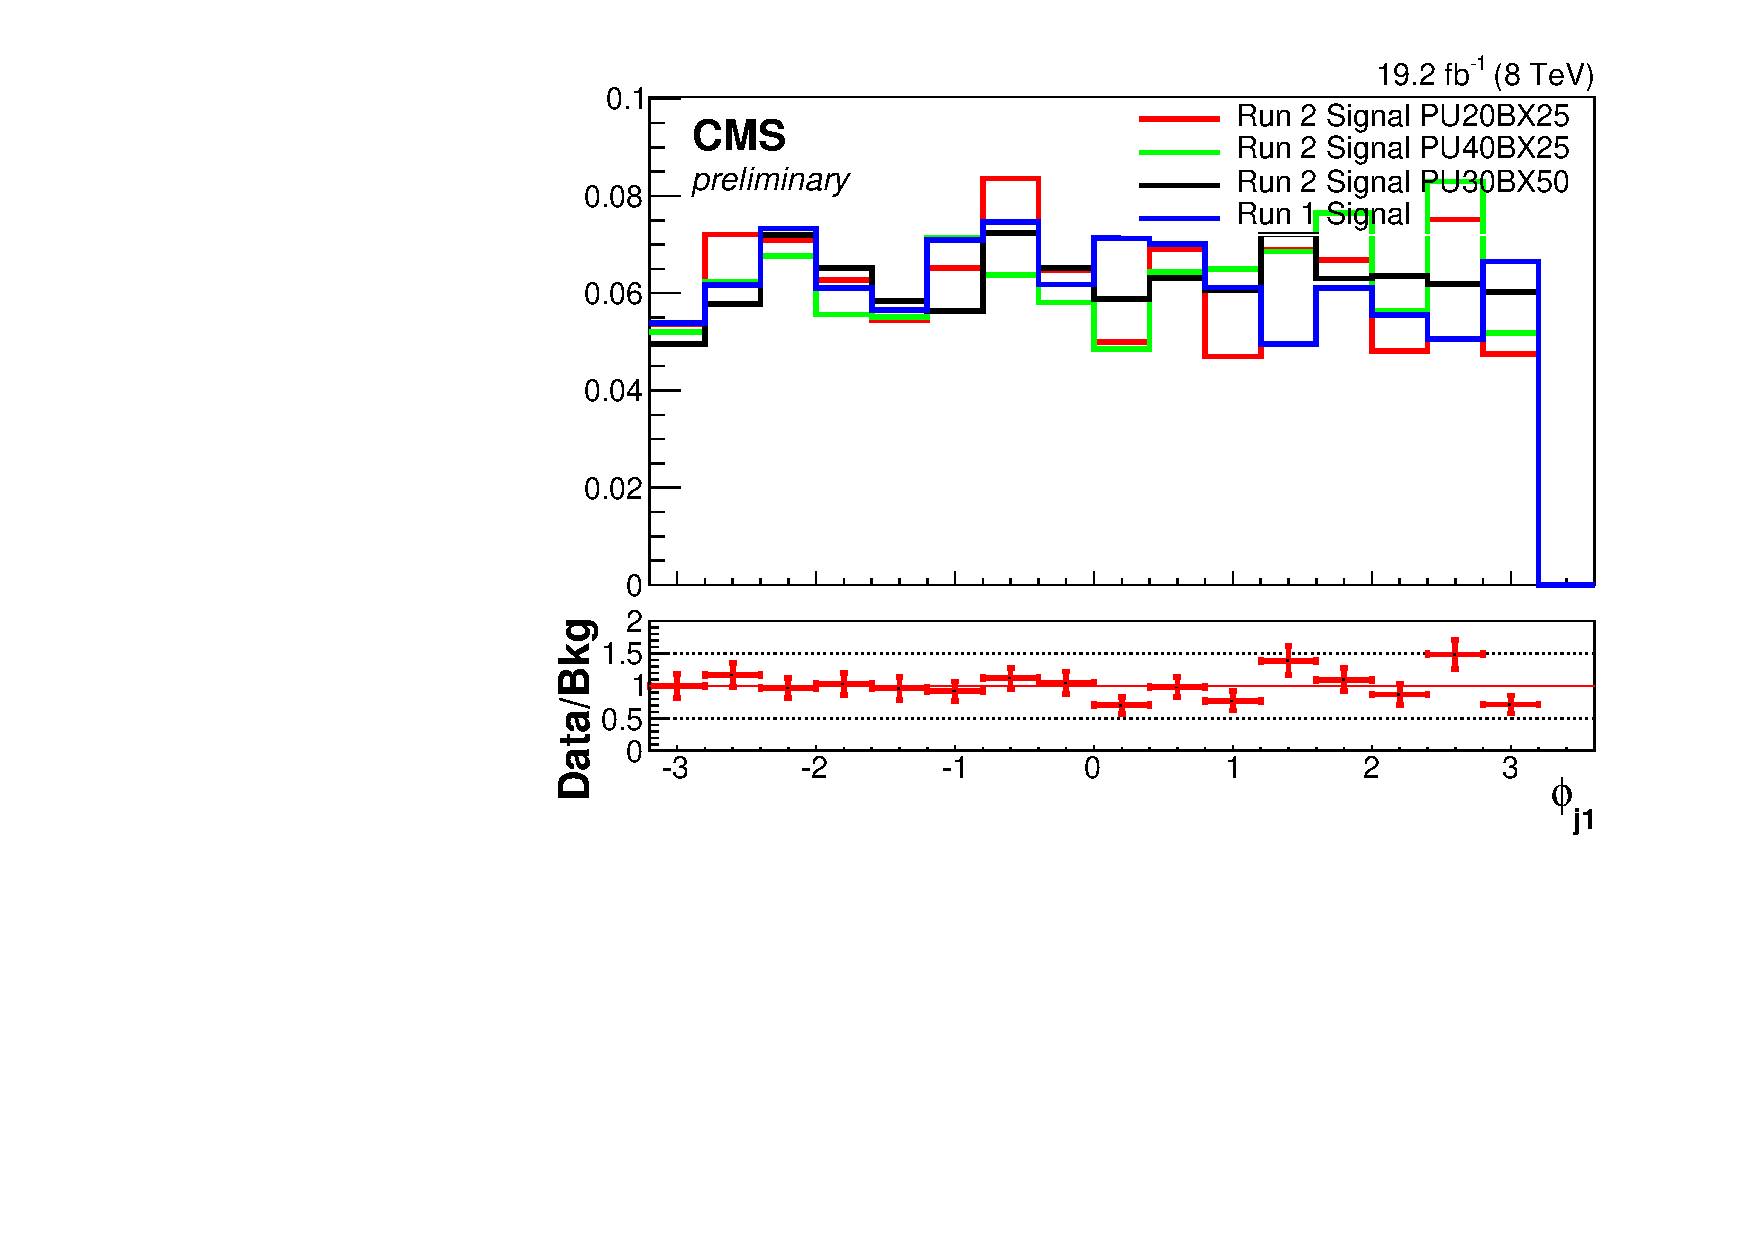
\includegraphics[width=.5\textwidth]{TalkPics/firstrun2mccontrolplots/output/nunu_norm_jet1_phi.pdf}
  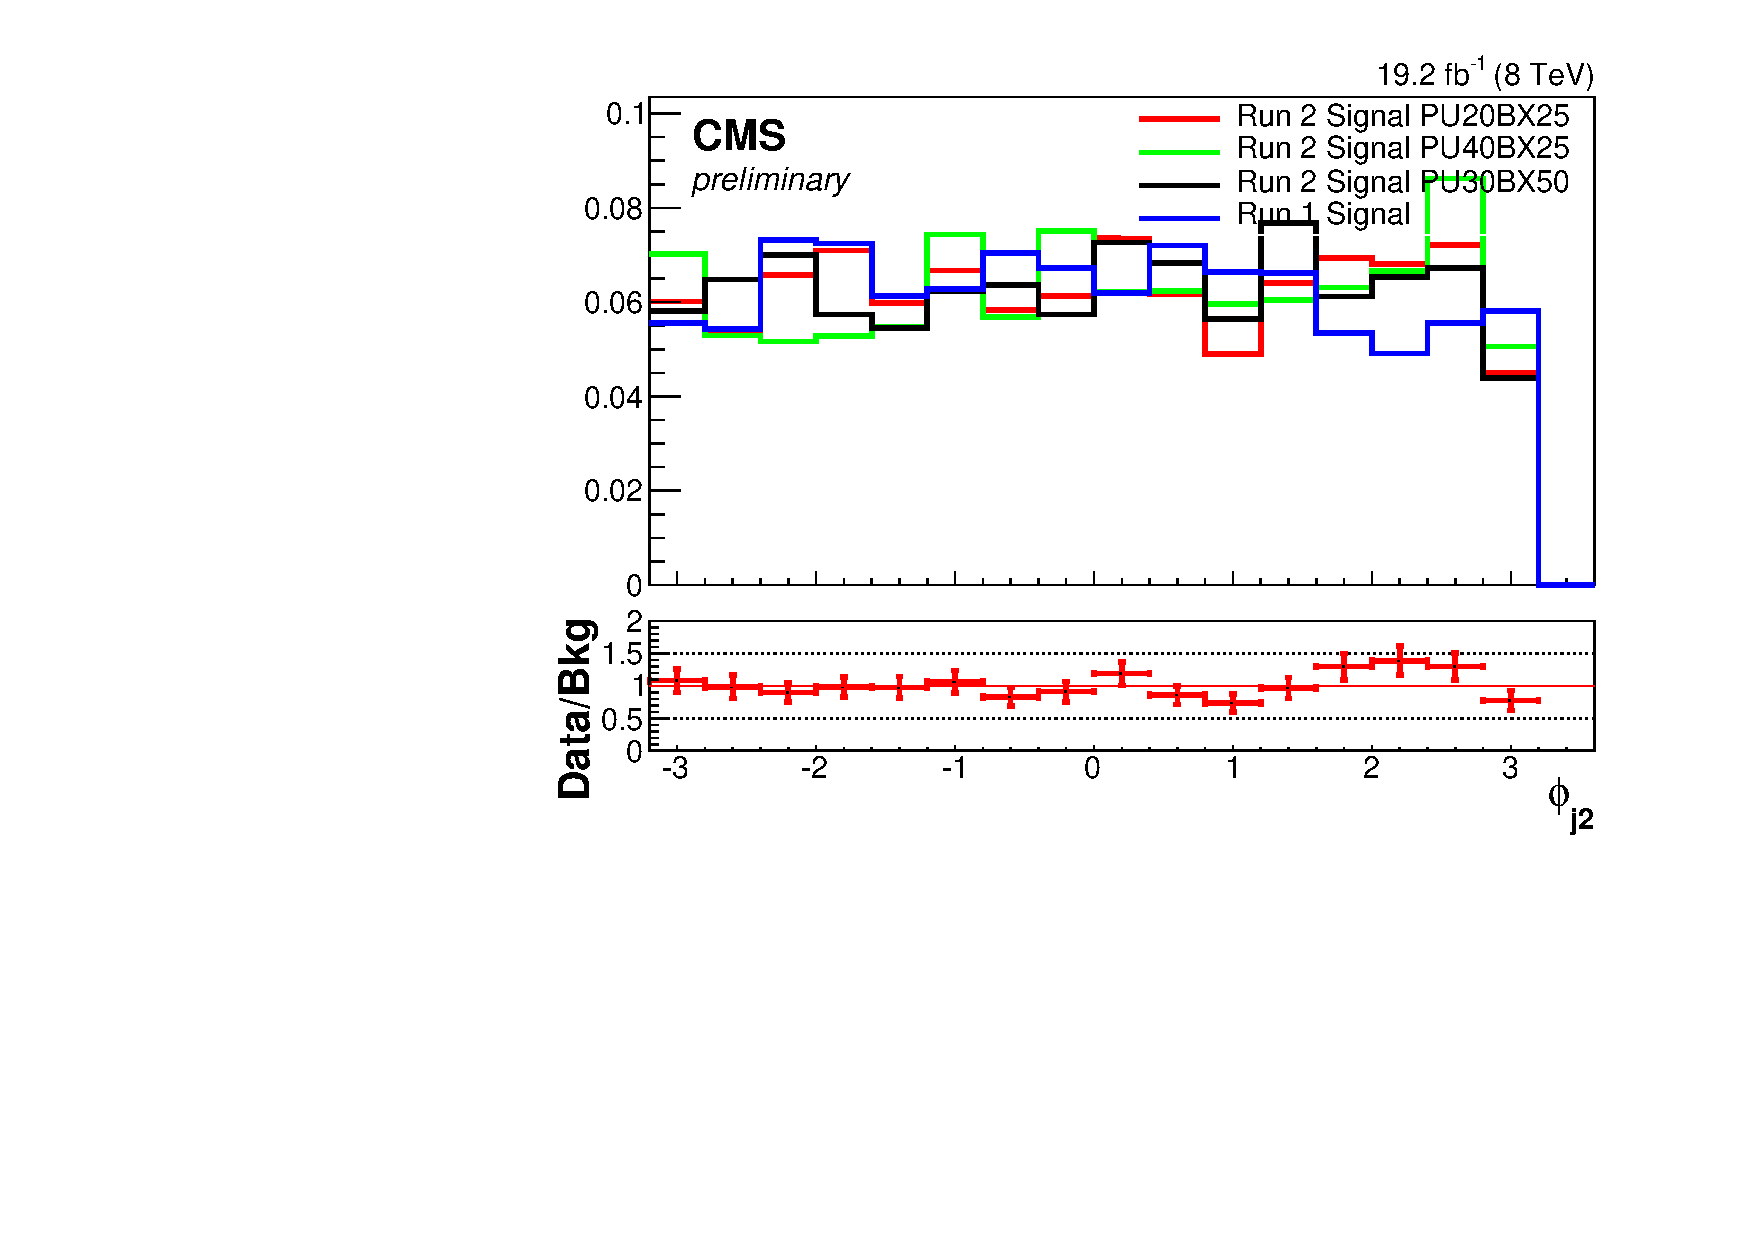
\includegraphics[width=.5\textwidth]{TalkPics/firstrun2mccontrolplots/output/nunu_norm_jet2_phi.pdf}
  \begin{block}{}
    \begin{itemize}
    \item $\phi$ distributions look comparable 
    \end{itemize}
  \end{block}
\end{frame}

\begin{frame}
  \frametitle{Signal comparison: run 1 vs run 2: Met}
  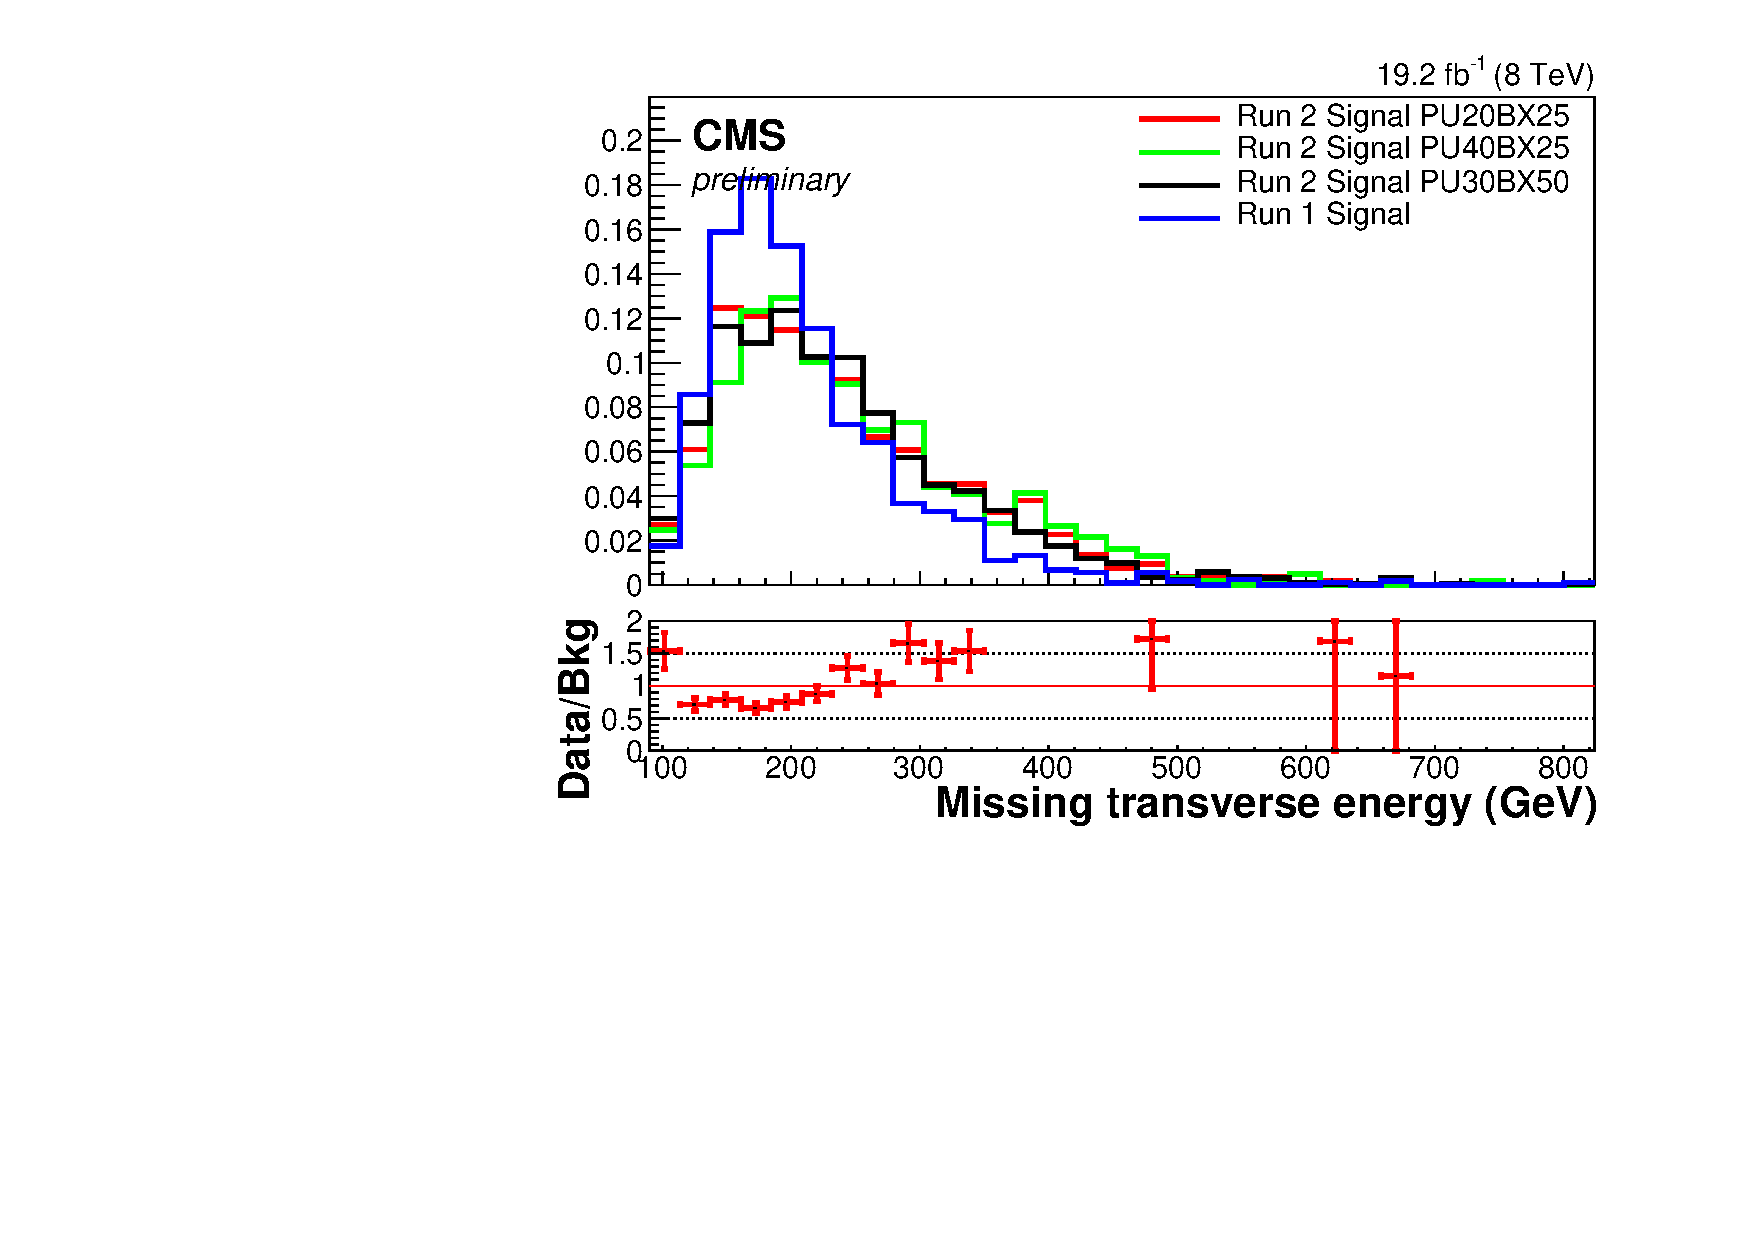
\includegraphics[width=.5\textwidth]{TalkPics/firstrun2mccontrolplots/output/nunu_norm_metnomuons.pdf}
  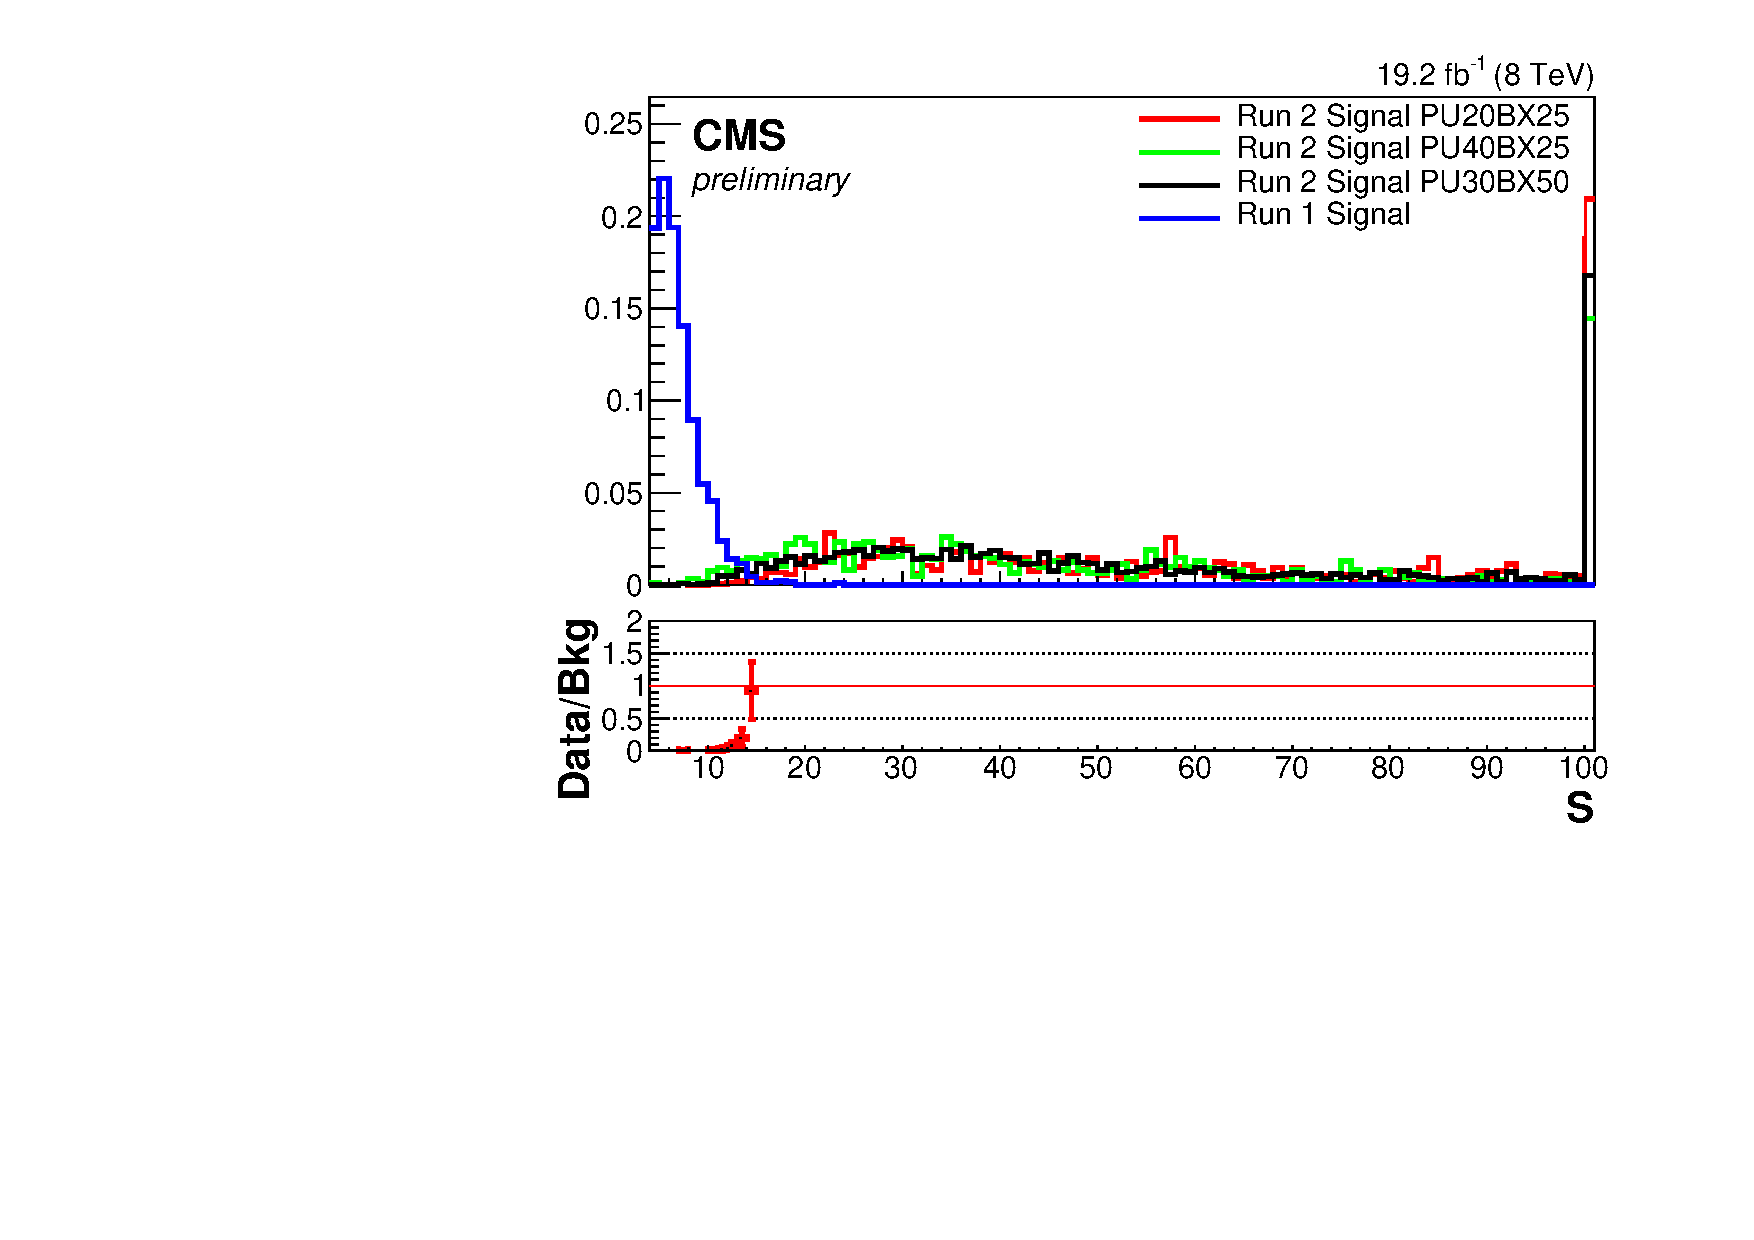
\includegraphics[width=.5\textwidth]{TalkPics/firstrun2mccontrolplots/output/nunu_norm_metnomu_significance.pdf}
  \begin{block}{}
    \begin{itemize}
    \item Met higher for run 2
    \item Met significance is a different variable in miniAOD to the one we used in run 1...
    \end{itemize}
  \end{block}
\end{frame}

\begin{frame}
  \frametitle{Signal comparison: run 1 vs run 2: $\Delta\phi$ variables}
  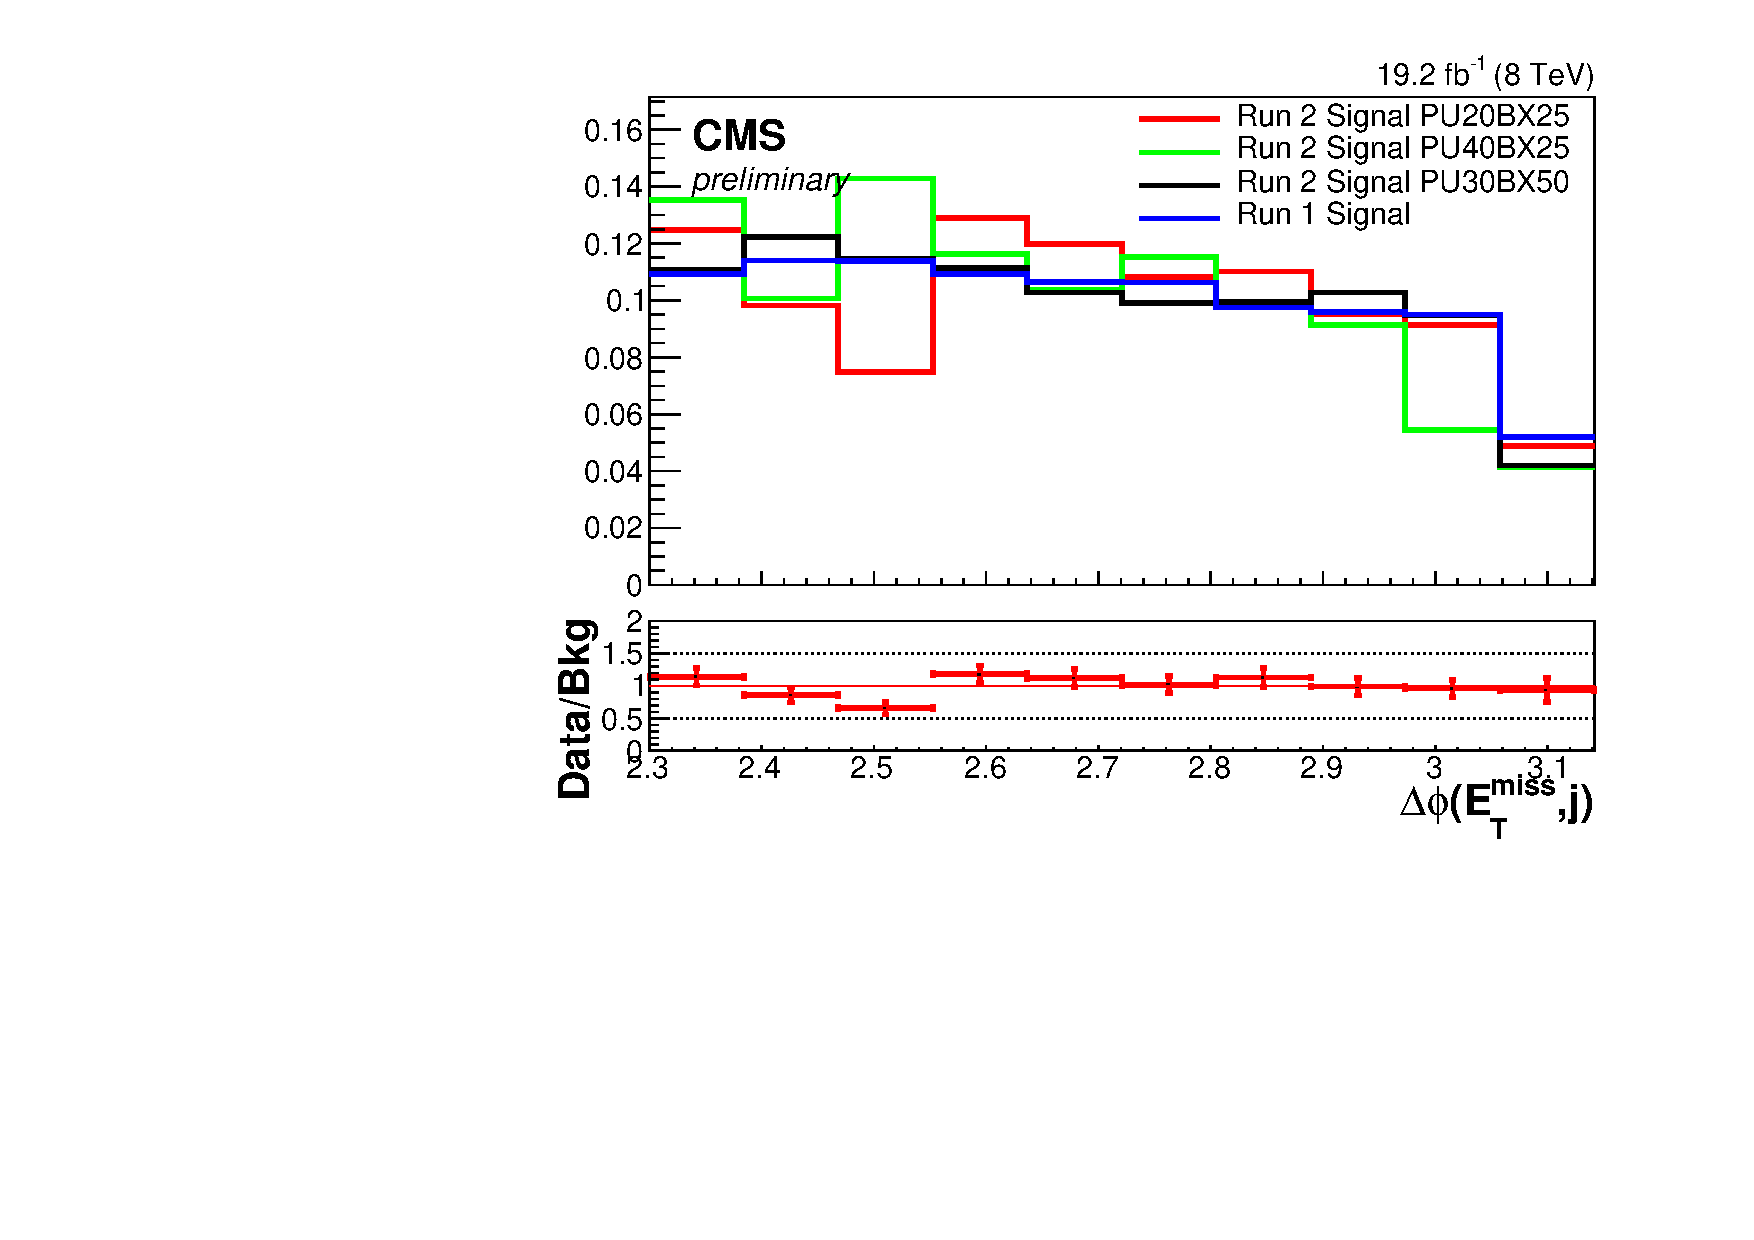
\includegraphics[width=.5\textwidth]{TalkPics/firstrun2mccontrolplots/output/nunu_norm_alljetsmetnomu_mindphi.pdf}
  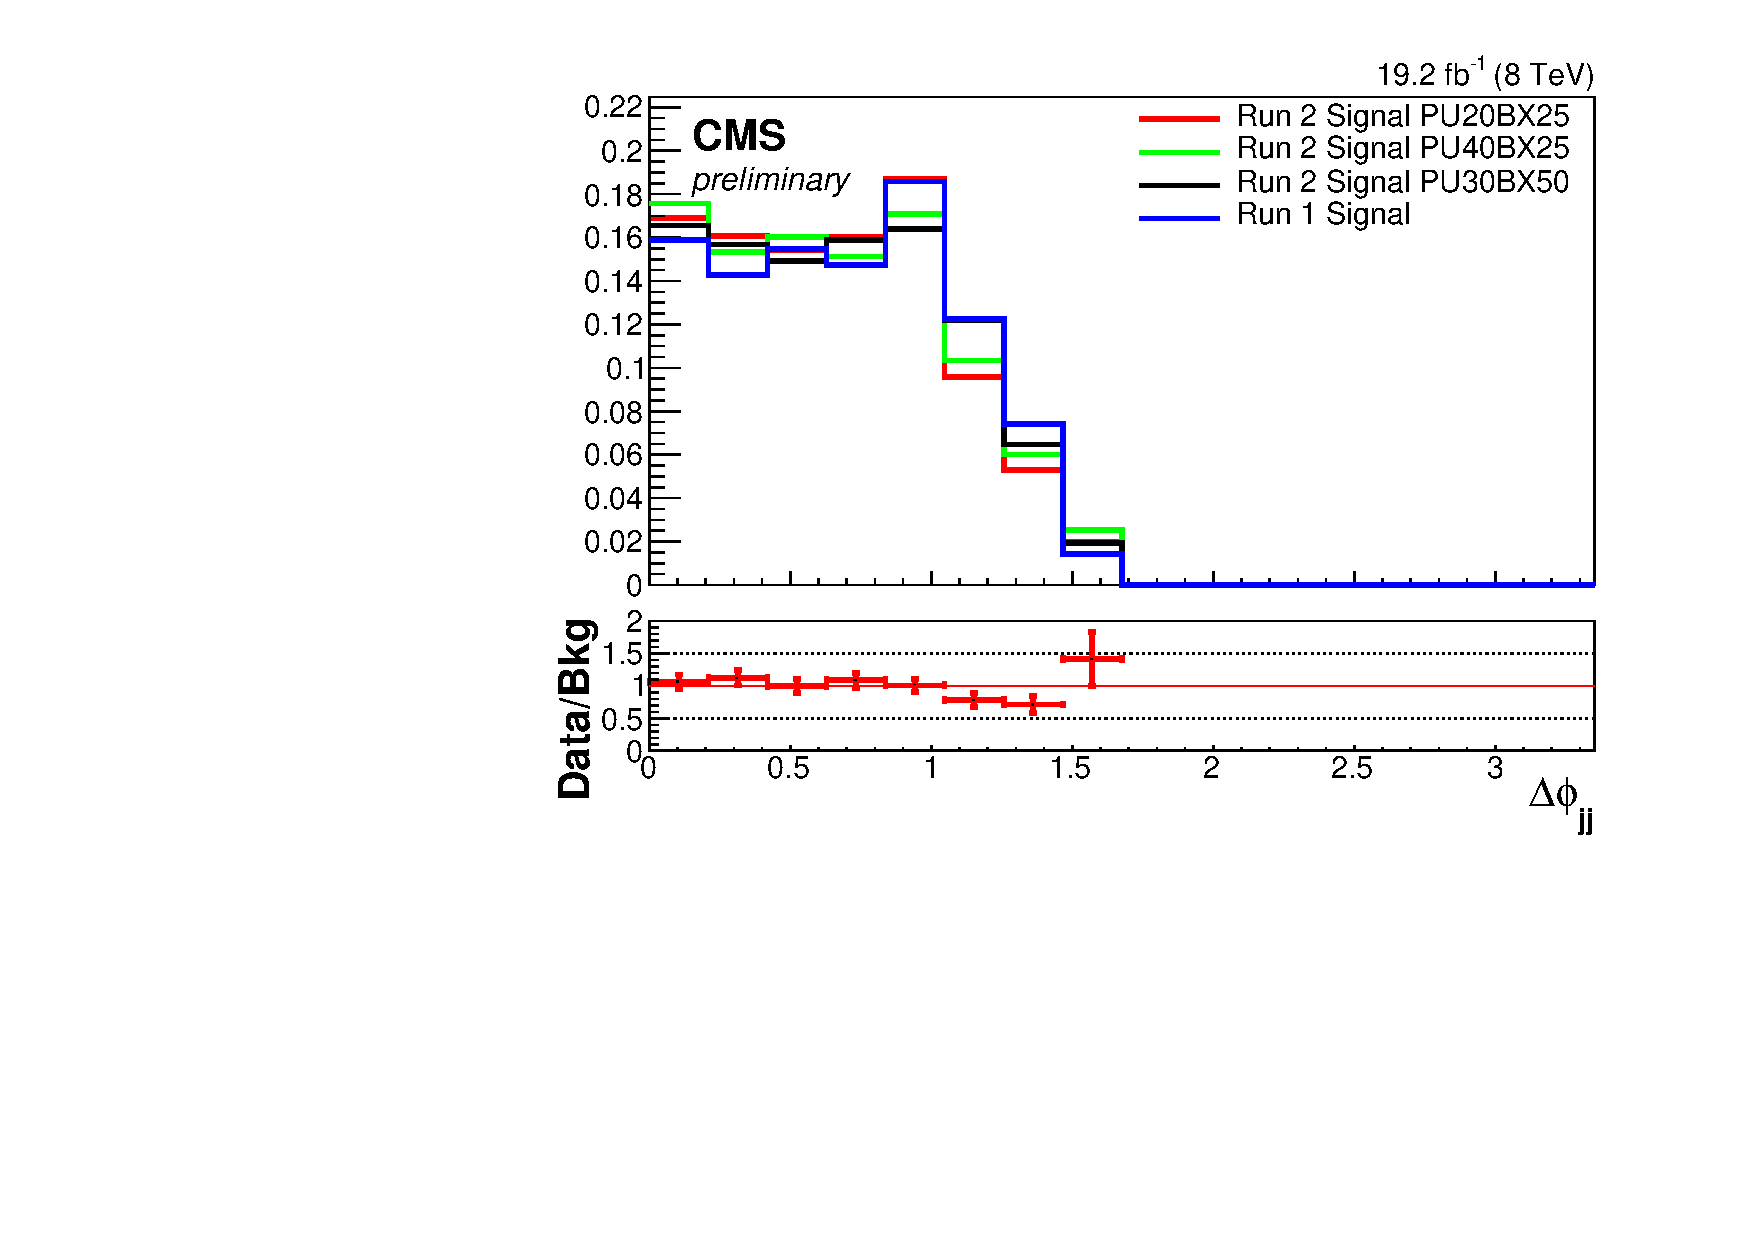
\includegraphics[width=.5\textwidth]{TalkPics/firstrun2mccontrolplots/output/nunu_norm_dijet_dphi.pdf}
  \begin{block}{}
    \begin{itemize}
    \item NB already cutting on jet-met $\Delta\phi$
    \item None the less distributions look quite similar
    \end{itemize}
  \end{block}
\end{frame}

\begin{frame}
  \frametitle{Signal comparison: run 1 vs run 2: dijet variables}
  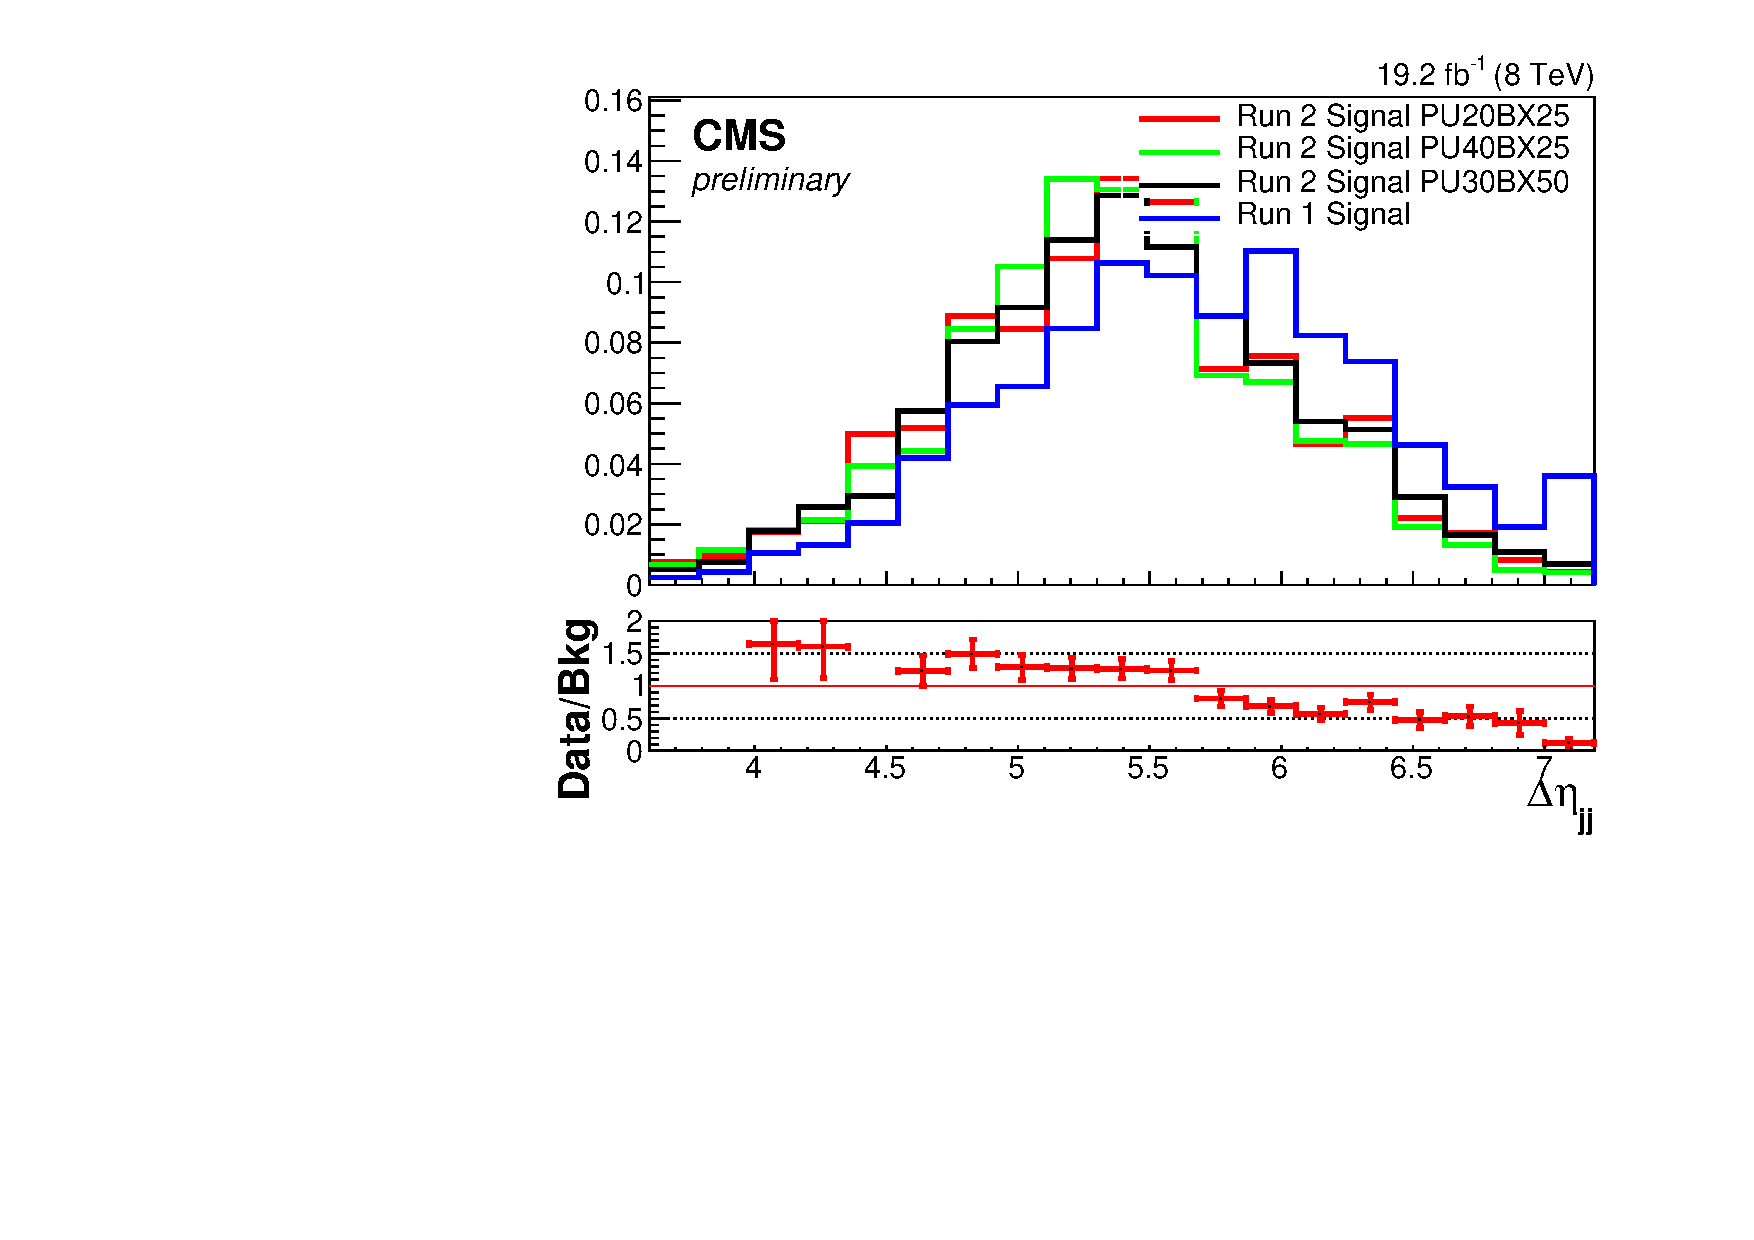
\includegraphics[width=.5\textwidth]{TalkPics/firstrun2mccontrolplots/output/nunu_norm_dijet_deta.pdf}
  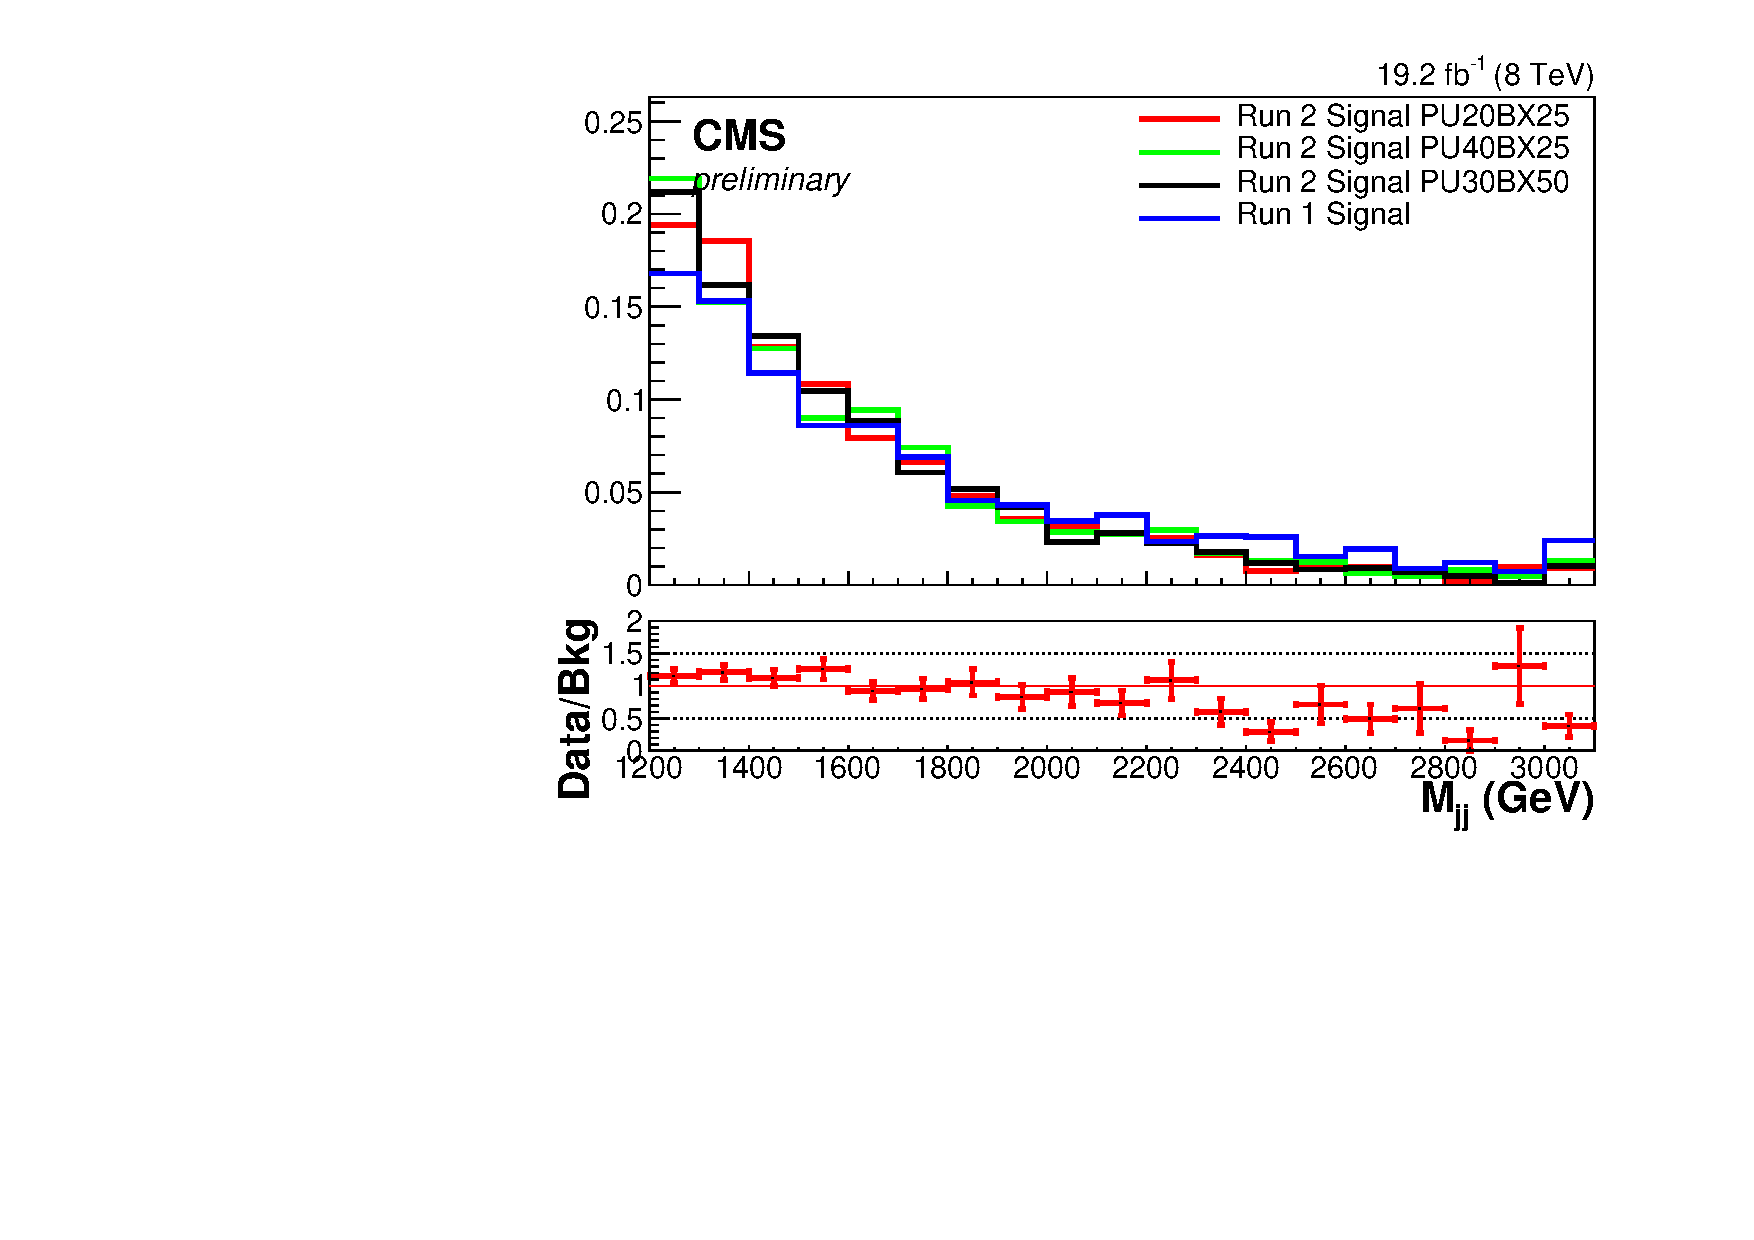
\includegraphics[width=.5\textwidth]{TalkPics/firstrun2mccontrolplots/output/nunu_norm_dijet_M.pdf}
   \begin{block}{}
     \begin{itemize}
     \item $\Delta\eta_{jj}$ smaller for run 2: could be due to $\eta$ ``ears''
     \item $M_{jj}$ also lower for run 2
     \item[-] Jet $p_{T}$ is higher in run 2, so must have less angular separation
     \item[-] $\Delta\phi_{jj}$ similar to run 1 so likely to be caused by lower $\Delta\eta_{jj}$
     \end{itemize}
   \end{block}
\end{frame}

\begin{frame}
  \frametitle{Signal comparison: run 1 vs run 2: N jets}
  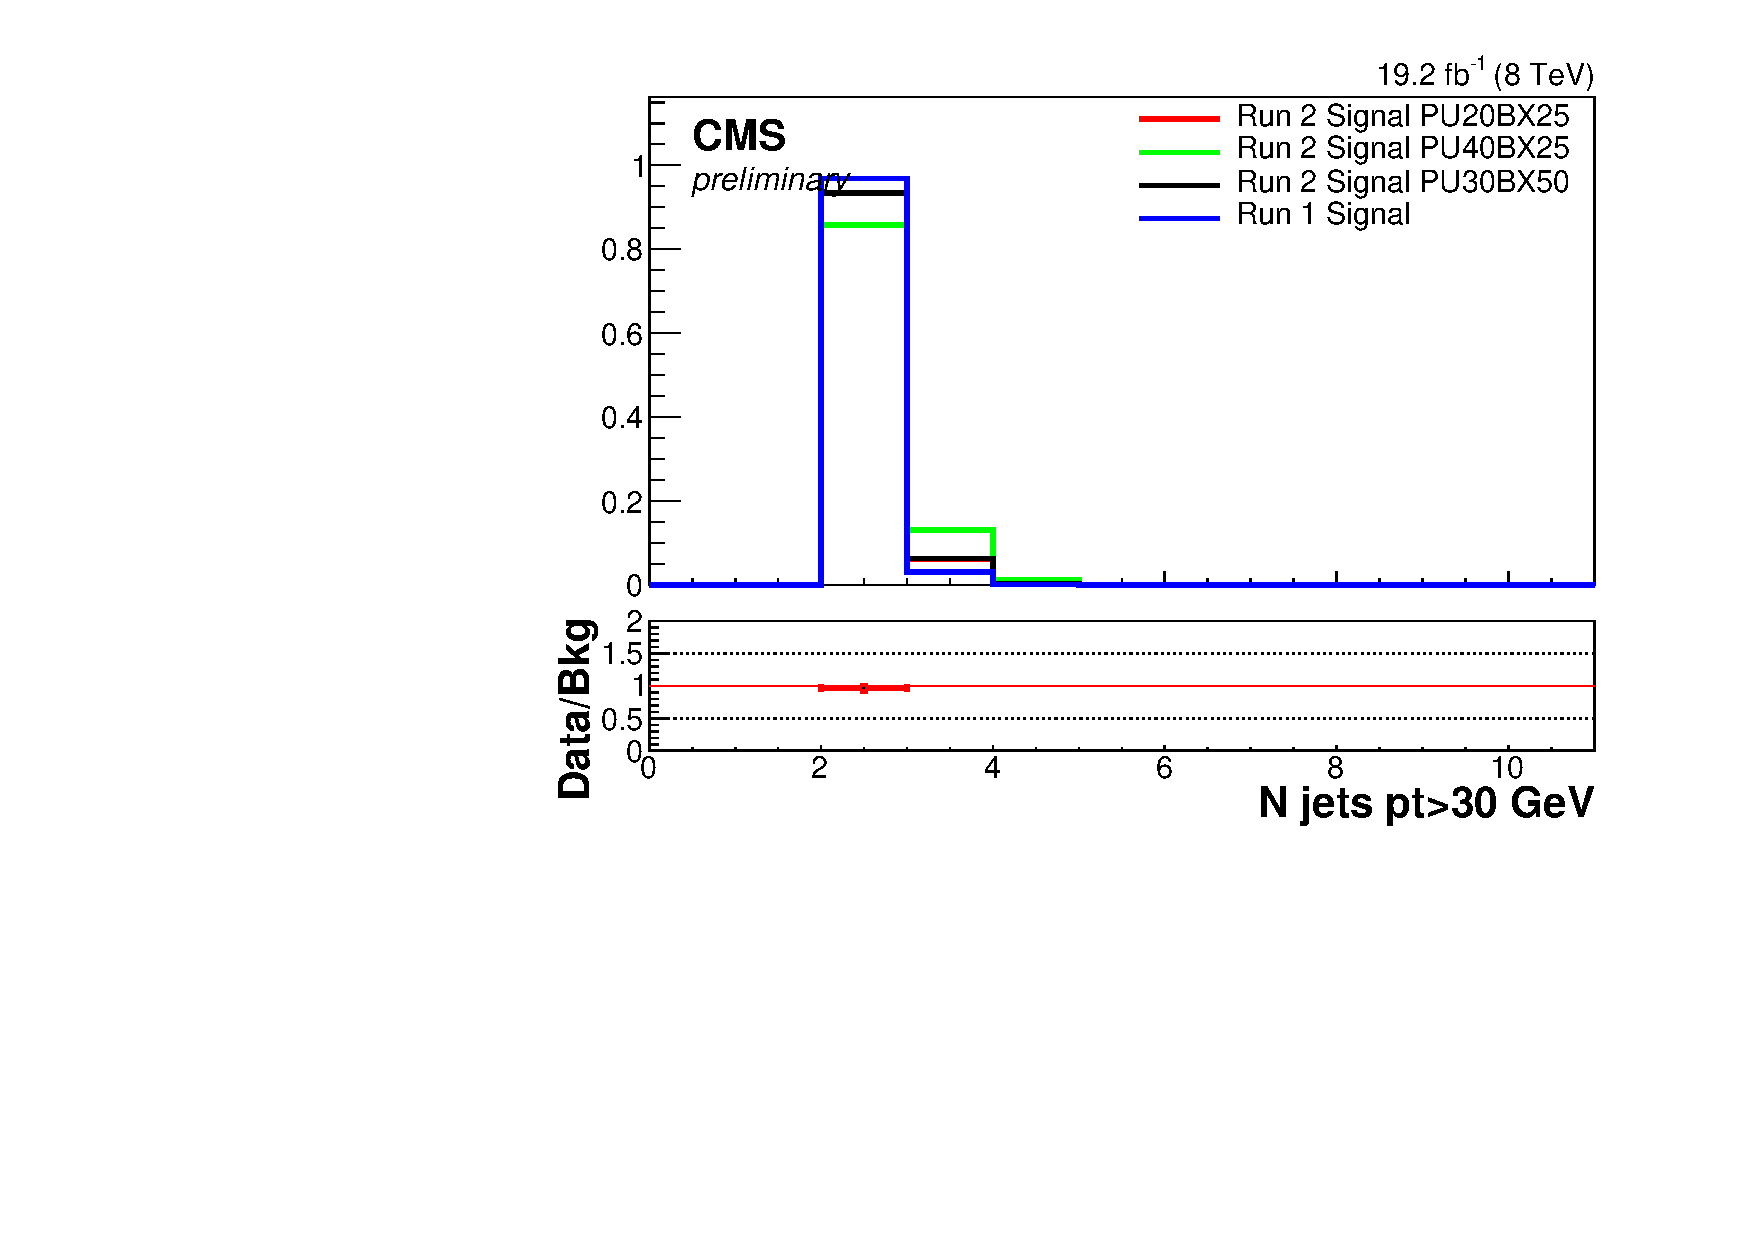
\includegraphics[width=.5\textwidth]{TalkPics/firstrun2mccontrolplots/output/nunu_norm_n_jets_30.pdf}
  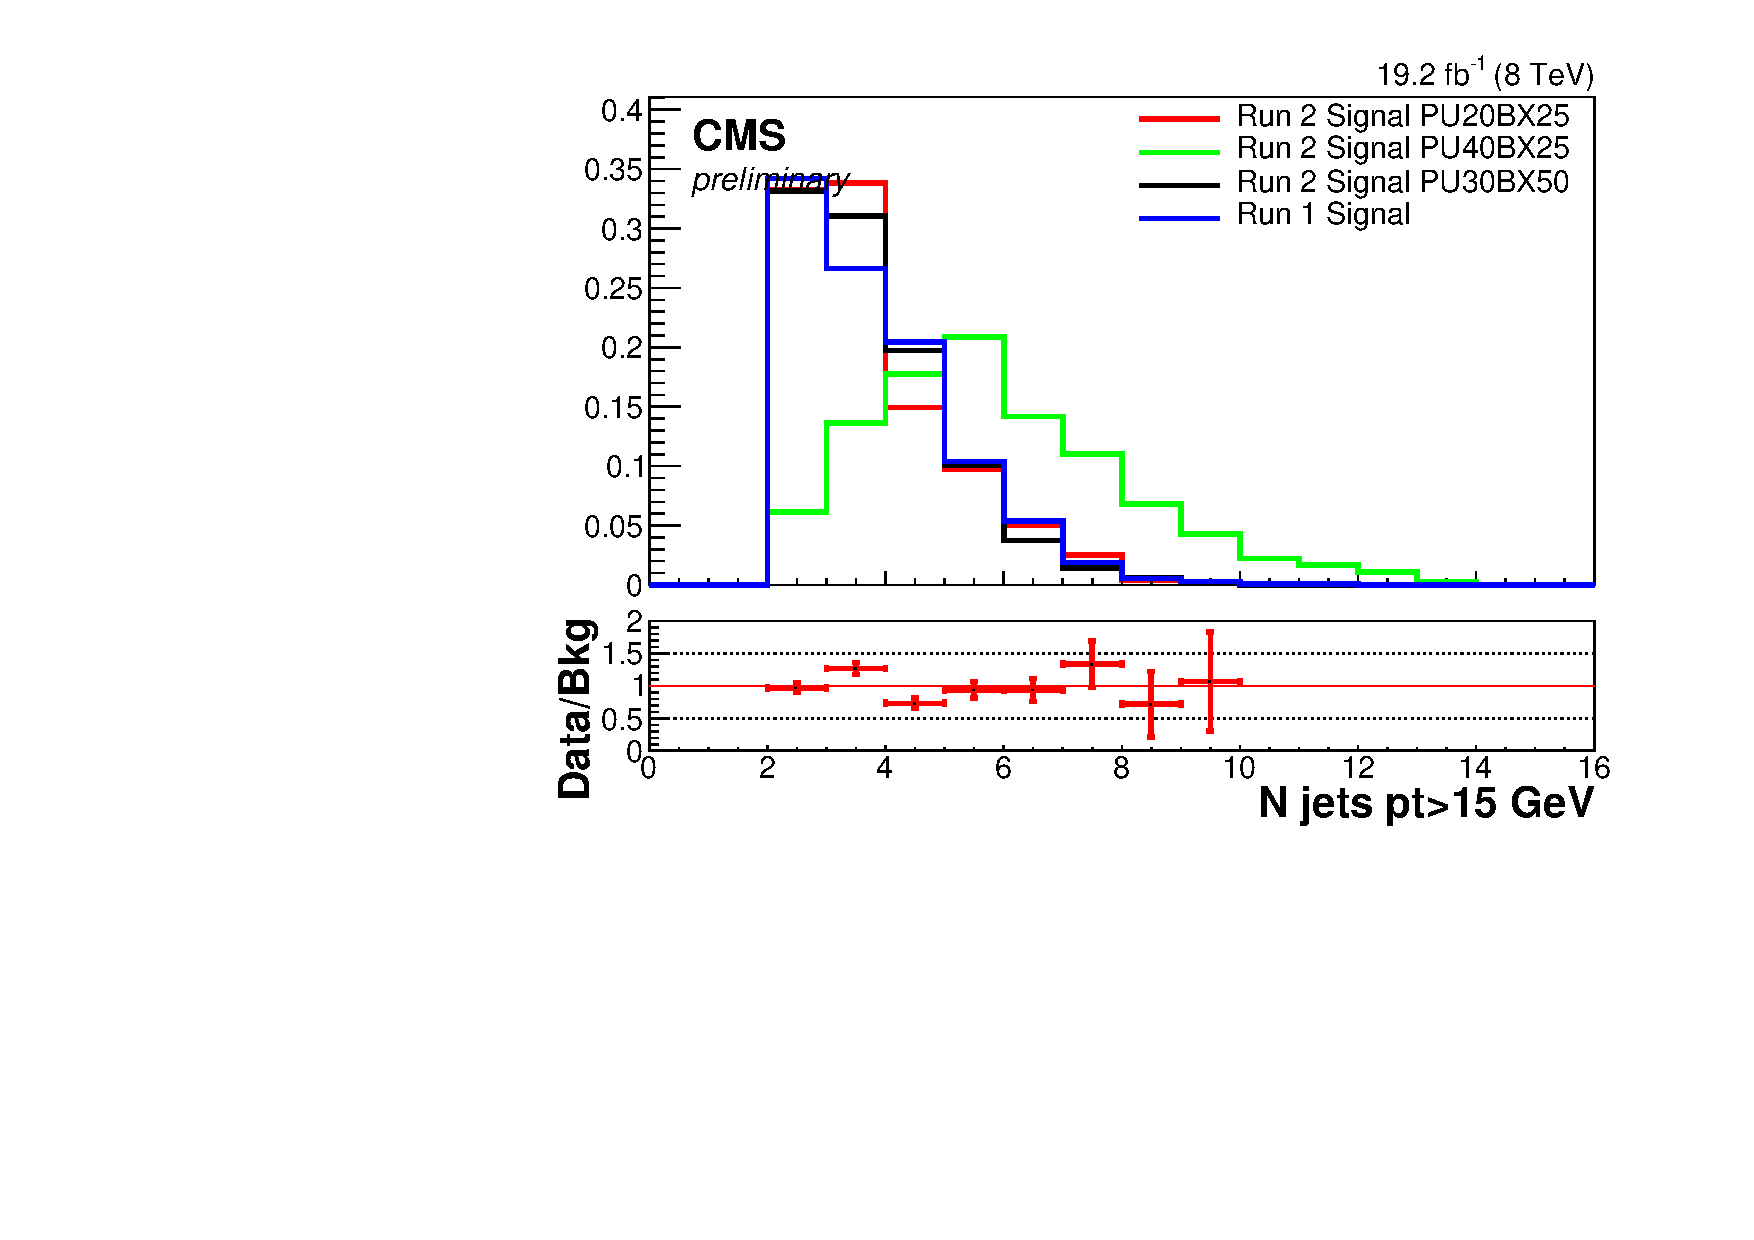
\includegraphics[width=.5\textwidth]{TalkPics/firstrun2mccontrolplots/output/nunu_norm_n_jets_15.pdf}
  \begin{block}{}
    \begin{itemize}
    \item Especially in right hand case higher pileup samples have a lot more jets per event as expected
    \end{itemize}
  \end{block}
\end{frame}


\begin{frame}
  \label{lastframe}
  \begin{block}{Summary}
    \begin{itemize}
    \item First signal MC comparisons between run 1 and run 2 performed
    \item Jet $\eta$ ``ears'' problem seen
    \item[-] to be improved in CMSSW\_7\_4\_2
    \end{itemize}
  \end{block}
  \begin{block}{Next steps}
    \begin{itemize}
    \item Look at QCD samples:
    \item[-] Only have PU20BX25
    \item[-] They are standard inclusive samples so won't model fake met
    \item Look at other regions:
    \item[-] e.g. parked analysis pre-selection region
    \end{itemize}
  \end{block}
\end{frame}

\begin{frame}
  \frametitle{Backup}
\end{frame}

\end{fmffile}
\end{document}
